% СПО ЛКС - TCP/IP
% Пынькин Д.А. (с) 2011
\documentclass[ignorenonframetext, hyperref={pdftex, unicode}]{beamer}
\usepackage{beamerthemesplit}

\usetheme{Pittsburgh}
\usecolortheme{dolphin}

\usepackage[russian]{babel}
\usepackage[utf8]{inputenc}
\usepackage[T1]{fontenc}
\usepackage{ulem}
%\usepackage{html}

\usepackage{verbatim}

\usepackage{tikz}
\usetikzlibrary{positioning,arrows}

\title[СПОЛКС (http://goo.gl/32cTB)]{Системое программное обеспечение локальных компьютерных сетей}
\author{Денис Пынькин}
\date{2011 -- 2012}
%\institution[БГУИР]{Белорусский государственный университет информатики и радиоэлектроники}
%\logo{
\includegraphics[width=1cm]{logo-kafEVM.png}}


\subtitle[TCP/IP]{Стек протоколов TCP/IP}

\begin{document}

\mode<all>{\begin{frame}
\titlepage
\begin{center}
e-mail: denis.pynkin@bsuir.by\\
\end{center}
\begin{center}
{\bfseries http://goo.gl/32cTB}

{\tiny СЧАСТЬЕ ДЛЯ ВСЕХ, ДАРОМ, И ПУСТЬ НИКТО НЕ УЙДЕТ ОБИЖЕННЫЙ!\\
(c)Стругацкие, Пикник на обочине}
\end{center}
\end{frame}
}

%
% Далее начинается сама презентация
%
%\section*{Введение}

\begin{frame}{Даты}
	\begin{block}{1975}
	Первый тест между двумя системами
	\end{block}
	\pause
	\begin{block}{1977}
	Тестовая сеть между тремя системами США, Великобритании и Норвегии
	\end{block}
	\pause
	\begin{block}{1978-1983}
	Тестируется 4 версии стека TCP/IP. И только в 3-й происходит разделение на протоколы TCP и IP.
	\end{block}
	\pause
	\begin{block}{Март 1982}
	US DoD объявляет стек TCP/IP стандартом для военных сетей.
	\end{block}
	\pause
	\begin{block}{01 января,  1983}
	День рождения Интернет -- именно в этот день Arpanet официально переключилась с NCP на TCP/IP 
	\end{block}
\end{frame}


\begin{frame}{Топология сети}
	\begin{columns}
	\column{0.3\textwidth}
	\vspace{5em}
	\begin{itemize}
		\item Прикладной
		\item Транспортный
		\item Межсетовой
		\item От хоста к сети
	\end{itemize}

	\column{0.7\textwidth}
	\begin{center}
		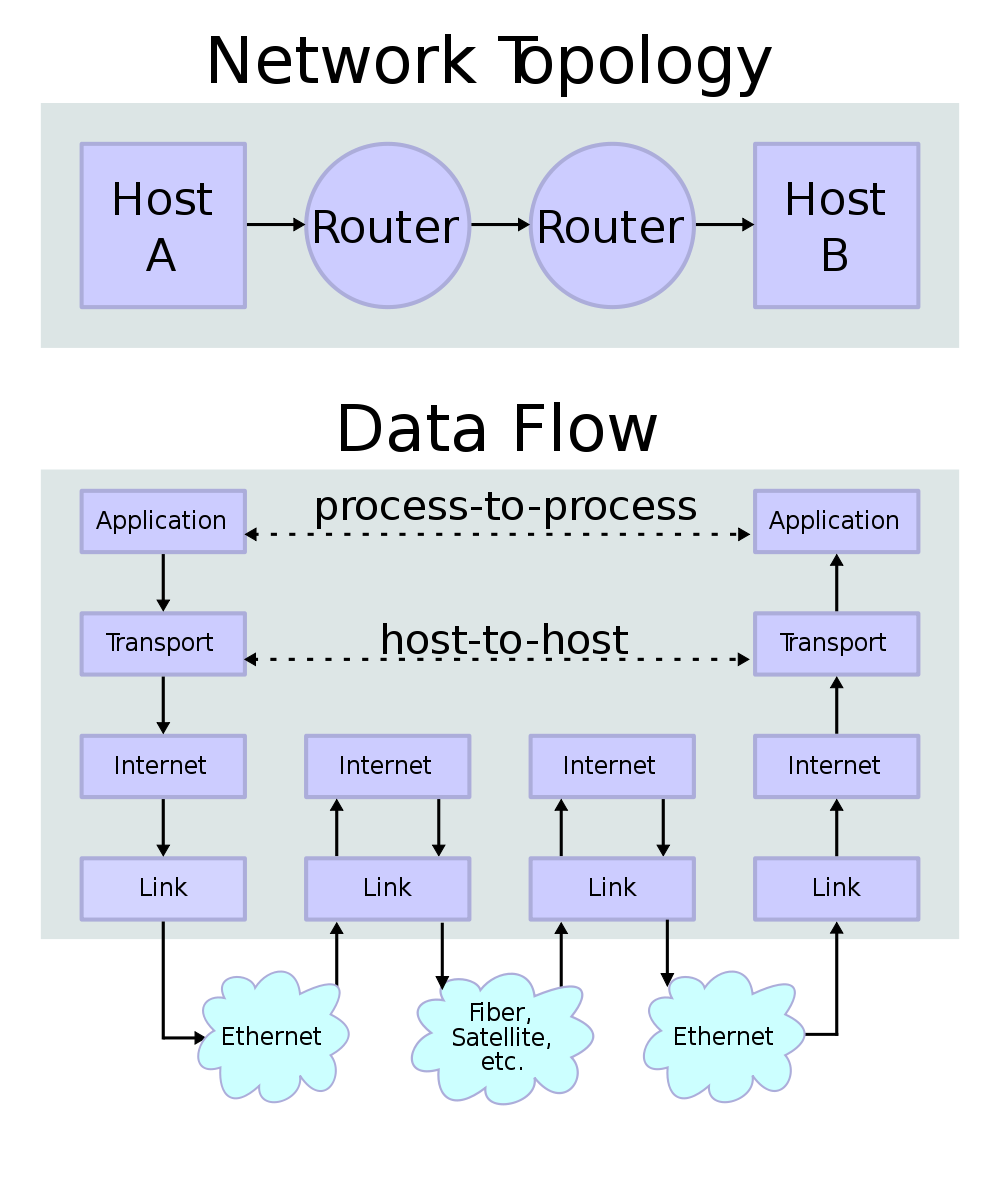
\includegraphics[height=0.9\textheight]{03-1000px-IP_stack_connections.png}
	\end{center}
	\end{columns}
\end{frame}

\begin{frame}{Стек TCP/IP}
	\begin{center}
		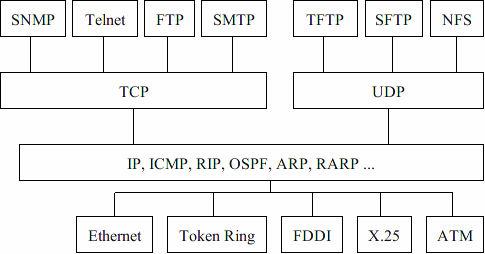
\includegraphics[width=1\textwidth]{03-TCP_IP.png}
	\end{center}
\end{frame}

\section[IP]{Межсетевой протокол IP}
\begin{frame}{Межсетевой протокол IP (RFC 791)}
	\begin{itemize}
		\item реализует обмен информации пакетами (IP-сегментами) (максимальный размер -- 65535 байт);
		\item является протоколом взаимодействия без установления логического соединения;
		\item для адресации узлов сети используется адрес длиной 4 байта;
		\item обеспечивает в случае необходимости фрагментацию IP-сегментов;
		\item IP-сегменты имеют конечное время жизни в сети;
		\item не гарантирует надежность доставки IP-сегментов адресату;
		\item не имеет средств управления интенсивностью передачи IP-сегментов посылающей стороной (flow control);
		\item не гарантирует правильную последовательность IP-сегментов на принимающей стороне.
	\end{itemize}
\end{frame}
\subsection{Заголовок}
\begin{frame}{Заголовок IP-сегмента}
	\begin{center}
		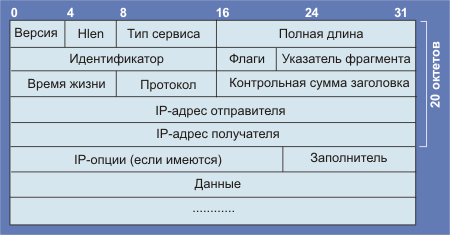
\includegraphics[width=1\textwidth]{03-ip_format.png}
	\end{center}

\end{frame}

\begin{frame}{Заголовок IP-сегмента: тип сервиса}
	\begin{center}
		
\includegraphics[height=0.1\textheight]{03-tos.png}
	\end{center}
	\begin{columns}
		\column{0.5\textwidth}
		Приоритет:
		\begin{itemize}
			\item 0 Обычный уровень
			\item 1 Приоритетный
			\item 2 Немедленный
			\item 3 Срочный
			\item 4 Экстренный
			\item 5 ceitic/ecp
			\item 6 Межсетевое управление
			\item 7 Сетевое управление
		\end{itemize}
		\column{0.5\textwidth}
		Формат поля TOS определен в документе RFC-1349.
		
		D=1 требует минимальной задержки,\\		
		T=1 - высокую пропускную способность,\\
		R=1 - высокую надежность,\\
		C=1 - низкую стоимость.
	\end{columns}
	\begin{center}в настоящее время определяется RFC2474 как\\«Differentiated Services»\end{center}
\end{frame}

\begin{frame}{Заголовок IP-сегмента: опции}
	\begin{center}
		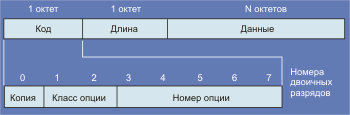
\includegraphics[height=0.2\textheight]{03-ip_option.png}
	\end{center}
	\scriptsize
	\begin{itemize}
		\item Конец списка опций. Используется,  если опции не укладываются в поле заголовка (смотри также поле "заполнитель")
		\item Никаких операций (используется для выравнивания октетов в списке опций)
		\item Ограничения,  связанные с секретностью (для военных приложений)
		\item Свободная маршрутизация. Используется для того,  чтобы направить дейтограмму по заданному маршруту
		\item Запись маршрута. Используется для трассировки
		\item Идентификатор потока. Устарело.
		\item Жесткая маршрутизация. Используется,  чтобы направить дейтограмму по заданному маршруту
		\item Временная метка Интернет
	\end{itemize}
	\normalsize
\end{frame}

\begin{frame}[fragile]{RFC 1071 -- вычисление контрольной суммы}
	\scriptsize	
\begin{lstlisting}[Language=C]
register long sum = 0;
while( count > 1 ){
/*  This is the inner loop */
  sum += * (unsigned short) addr++;
  count -= 2;
}

/*  Add left-over byte,  if any */
if( count > 0 )
  sum += * (unsigned char *) addr;

/*  Fold 32-bit sum to 16 bits */
while (sum>>16)
  sum = (sum & 0xffff) + (sum >> 16);

checksum = ~sum;
\end{lstlisting}
	\normalsize
\end{frame}

\subsection{Адрес}
\begin{frame}{Адреса IPv4}
IP-адрес представляет собой четырехбайтовое число,  старшие (крайние левые) биты которого определяют класс IP-адреса.
	\begin{center}
		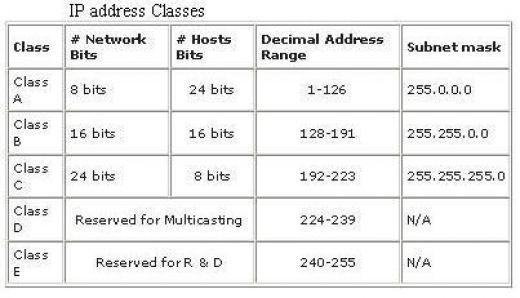
\includegraphics[height=0.6\textheight]{03-ip_class.png}
	\end{center}

\end{frame}

\begin{frame}{Специальные IP адреса}

	\scriptsize
	\begin{table}[ht]
	\centering
	\begin{tabular}[c]{r|l|c}
CIDR address block & Description & Reference \\
	\hline
0.0.0.0/8 &	Current network (only valid as source address)&	RFC 1700\\
10.0.0.0/8 &	Private network &		RFC 1918\\
127.0.0.0/8 &		Loopback &	RFC 5735\\
169.254.0.0/16 &	Link-Local &	RFC 3927\\
172.16.0.0/12 &	Private network &		RFC 1918\\
192.0.0.0/24 &	Reserved (IANA) &		RFC 5735\\
192.0.2.0/24 &	TEST-NET-1,  Documentation and example code &		RFC 5735\\
192.88.99.0/24 &	IPv6 to IPv4 relay &	RFC 3068\\
192.168.0.0/16 &	Private network &		RFC 1918\\
198.18.0.0/15 &	Network benchmark tests &		RFC 2544\\
198.51.100.0/24 &		TEST-NET-2,  Documentation and examples &		RFC 5737\\
203.0.113.0/24 &	TEST-NET-3,  Documentation and examples &		RFC 5737\\
224.0.0.0/4 &		Multicasts (former Class D network) &		RFC 3171\\
240.0.0.0/4 &		Reserved (former Class E network) &	RFC 1700\\
255.255.255.255 &		Broadcast &	RFC 919
	\end{tabular}
	\caption{Специальные адреса}
	\end{table}
	\normalsize
\end{frame}

\subsection{Фрагментация}
\begin{frame}{Фрагментация IP}
Для того,  чтобы существовала возможность передачи IP-сегментов через сети различного типа,  
межсетевой протокол обеспечивает адаптацию их размера к требованиям каждой сети. Это дает возможность,  
например,  IP-сегментам,  порожденным в сети на базе Ethernet (максимальный размер кадра -- 1526 байт),  
беспрепятственно перемещаться до адресата по сети на базе X.25 (максимальный размер кадра - 128 байт). 

Изменение размера IP-сегмента в процессе перемещения по сети может быть связано и с соображениями эффективности передачи.	
\end{frame}

\begin{frame}{Фрагментация IP}
Каждый IP-фрагмент представляет собой полноценный IP-сегмент со своим собственным IP-заголовком. 
Однако заголовки всех IP-фрагментов содержат одинаковый идентификатор,  
совпадающий с идентификатором исходного IP-сегмента. Это позволяет распознавать все IP-фрагменты,  относящиеся к одному исходному IP-сегменту.	
\end{frame}

\begin{frame}{Фрагментация IP}
	\begin{center}
		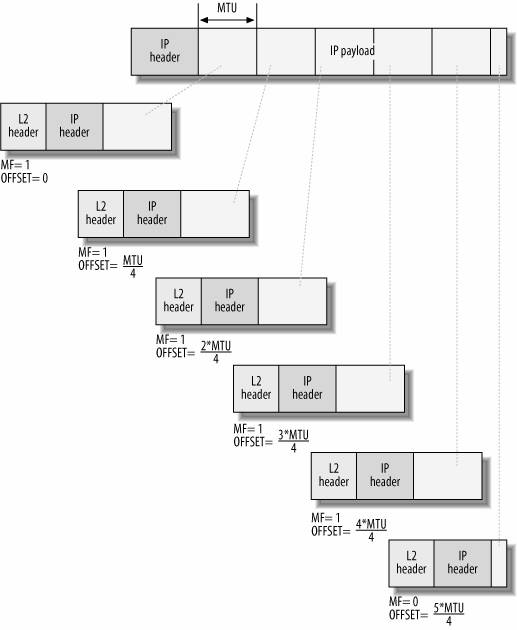
\includegraphics[height=0.8\textheight]{03-ip_fragmentation.png}
	\end{center}
\end{frame}

\begin{frame}{Фрагментация IP}
IP-модуль на принимающем IP-фрагменты узле в ситуации,  когда он должен транслировать IP-сегмент далее по сети,  имеет три варианта действий с фрагментами:
	\begin{itemize}
		\item переслать IP-фрагменты далее неизменными;
		\item разбить (если в этом есть необходимость) полученные IP-фрагменты на более короткие IP-фрагменты;
		\item восстановить исходный IP-сегмент из фрагментов.
	\end{itemize}
 В работе с IP-фрагментами на принимающей стороне используется специальный таймер,  который с приходом первого фрагмента IP-сегмента устанавливается в исходное состояние (для UNIX-реализаций это,  обычно,  30 сек) и начинает обратный счет.
\end{frame}

\section{ICMP}
\begin{frame}{Протокол ICMP}
	Протокол передачи команд и сообщений об ошибках \\
	(ICMP -- internet control message protocol, RFC-792)\\
	\pause
	\bigskip
ICMP позволяет маршрутизатору либо конечному узлу сообщить узлу-отправителю об ошибках,  
с которыми машрутизатор столкнулся при передаче какого-либо IP-пакета от данного конечного узла.
\end{frame}

\begin{frame}{ICMP только для конечных узлов}
Управляющие сообщения ICMP не могут направляться промежуточному маршрутизатору,
 который участвовал в передаче пакета,  с которым возникли проблемы,  так как для такой посылки нет адресной информации - пакет несет в себе только адрес источника и адрес назначения,  не фиксируя адреса промежуточных маршрутизаторов.
\end{frame}

\begin{frame}{Спасение утопающих -- дело рук самих утопающих!}
	Протокол ICMP - это протокол сообщения об ошибках,  а не протокол коррекции ошибок.\\
	\bigskip
	Конечный узел может предпринять некоторые действия для того,  чтобы ошибка больше не возникала,  но эти действия протоколом ICMP не регламентируются.
\end{frame}

\begin{frame}{ICMP и IP}
	ICMP-протокол сообщает об ошибках в IP-дейтограммах,  но не дает информации об ошибках в самих ICMP-сообщениях.\\
	\pause
	\bigskip
	ICMP использует IP,  а IP-протокол должен использовать ICMP.\\
	\pause
	\bigskip
	В случае ICMP-фрагментации сообщение об ошибке будет выдано только один раз на дейтограмму,  даже если ошибки были в нескольких фрагментах.	
\end{frame}

\begin{frame}{Задачи ICMP}
	\begin{itemize}
		\item передача отклика на пакет или эхо на отклик;
		\item контроль времени жизни дейтограмм в системе;
		\item реализует переадресацию пакета;
		\item выдает сообщения о недостижимости адресата или о некорректности параметров;
		\item формирует и пересылает временные метки;
		\item выдает запросы и отклики для адресных масок и другой информации.
	\end{itemize}
\end{frame}

\begin{frame}
ICMP-сообщения об ошибках не выдаются:
	\begin{itemize}
		\item на ICMP-сообщение об ошибке;
		\item При мультикастинг или широковещательной адресации;
		\item Для фрагмента дейтограммы (кроме первого);
		\item Для дейтограмм,  чей адрес отправителя является нулевым,  широковещательным или мультикастинговым.
	\end{itemize}
\end{frame}

\begin{frame}{Заголовок ICMP}
	\begin{center}
		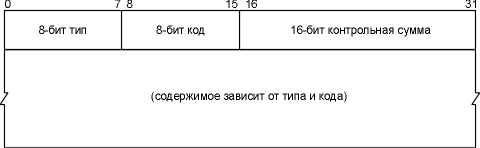
\includegraphics[height=0.4\textheight]{03-icmp_header.png}\\
		\pause
		\bigskip
		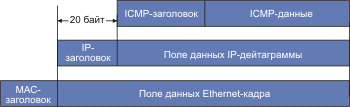
\includegraphics[height=0.4\textheight]{03-icmp_incapsulation.png}
	\end{center}
\end{frame}

\subsection{Типы сообщений}
\begin{frame}{Тип 0 -- Эхо-ответ (ping-отклик)}
	\scriptsize
	\begin{table}[ht]
	\centering
	\begin{tabular}[c]{r|l}
Код & Описание \\
	\hline
		0 & Эхо-ответ (ping-отклик)\\
	\end{tabular}
	\end{table}
	\normalsize
\end{frame}

\begin{frame}{Тип 3 -- Адресат недоступен}
	\scriptsize
	\begin{table}[ht]
	\centering
	\begin{tabular}[c]{r|l}
Код & Описание \\
	\hline
		0 & Сеть недостижима\\
		1 & ЭВМ не достижима\\
		2 & Протокол не доступен\\
		3 & Порт не доступен\\
		4 & Необходима фрагментация сообщения\\
		5 & Исходный маршрут вышел из строя\\
		6 & Сеть места назначения не известна\\
		7 & ЭВМ места назначения не известна\\
		8 & Исходная ЭВМ изолирована\\
		9 & Связь с сетью места назначения административно запрещена\\
		10 & Связь с ЭВМ места назначения административно запрещена\\
		11 & Сеть не доступна для данного вида сервиса\\
		12 & ЭВМ не доступна для данного вида сервиса\\
		13 & Связь административно запрещена с помощью фильтра.\\
		14 & Нарушение старшинства ЭВМ\\
		15 & Дискриминация по старшинству\\
	\end{tabular}
	\end{table}
	\normalsize
\end{frame}

\begin{frame}{Тип 5 - Переадресовать (изменить маршрут)}
	\scriptsize
	\begin{table}[ht]
	\centering
	\begin{tabular}[c]{r|l}
Код & Описание \\
	\hline
	0 & Переадресовать дейтаграмму в сеть (устарело)\\
	1 &	Переадресовать дейтаграмму на ЭВМ\\
	2 &	Переадресовать дейтаграмму для типа сервиса (tos) и сети\\
	3 & Переадресовать дейтаграмму для типа сервиса и ЭВМ\\
	\end{tabular}
	\end{table}
	\normalsize
\end{frame}

\begin{frame}{Тип 8 -- Эхо-запрос}
	\scriptsize
	\begin{table}[ht]
	\centering
	\begin{tabular}[c]{r|l}
Код & Описание \\
	\hline
		0 & Эхо запрос (ping-запрос)\\
	\end{tabular}
	\end{table}
	\normalsize
\end{frame}

\begin{frame}{Тип 11 -- Превышение временного интервала (для дейтаграммы время жизни истекло) (ttl=0)}
	\scriptsize
	\begin{table}[ht]
	\centering
	\begin{tabular}[c]{r|l}
Код & Описание \\
	\hline
		0 & при передаче\\
		1 & при сборке (случай фрагментации)\\
	\end{tabular}
	\end{table}
	\normalsize
\end{frame}

\begin{frame}{Тип 12 -- Проблема с параметрами дейтаграммы}
	\scriptsize
	\begin{table}[ht]
	\centering
	\begin{tabular}[c]{r|l}
Код & Описание \\
	\hline
		0 & Ошибка в ip-заголовке\\
		1 & Отсутствует необходимая опция\\
	\end{tabular}
	\end{table}
	\normalsize
\end{frame}

\begin{frame}{Там еще много подозрительных типов!}
	\scriptsize
	\begin{table}[ht]
	\centering
	\begin{tabular}[c]{r|l}
Тип & Описание \\
	\hline
4 & Сдерживание источника (отключение источника при переполнении очереди)\\
9 & Объявление маршрутизатора\\
10 & Запрос маршрутизатора\\
13 & Запрос метки времени\\
14 & Ответ с меткой времени\\
15 & Информационный запрос\\
16 & Информационный ответ\\
17 & Запрос адресной маски (RFC-950)\\
18 & Отклик на запрос адресной маски (RFC-950)\\
30 & Трассировка маршрута (RFC-1393)\\
31 & Ошибка преобразования датаграммы (RFC-1475)\\
32 & Перенаправление для мобильного узла\\
33 & IPv6 Where-Are-You (где вы находитесь)\\
34 & IPv6 I-Am-Here (я здесь)\\
35 & Запрос перенаправления для мобильного узла\\
36 & Отклик на запрос перенаправления для мобильного узла\\
37 & Запрос доменного имени (Domain Name Request)\\
38 & Ответ на запрос доменного имени (Domain Name Reply)\\
39 & SKIP\\
40 & Photuris\\
	\end{tabular}
	\end{table}
	\normalsize
\end{frame}

\mode<all>{\begin{frame}{}
\Huge
\begin{center}
	Спасибо за внимание!
	\bigskip
	Вопросы?
\end{center}
\normalsize
\end{frame}
}

\end{document}
%Конец файла
